% ycb1-fig-skeleton-divisions. Labels from notes block ycb1-hl-human-body-introduction,
% "Skeletal divisions" bullet (checked in pass 4).
\documentclass[border=6pt]{standalone}
% Shared preamble for the YCB1 line diagrams (standalone TikZ, XeTeX). Black and white only; labels come from
% the checked notes block named in each diagram file. Build: make_figures.bat in this folder.
\usepackage{fontspec}
\setmainfont{Segoe UI}
\usepackage{tikz}
\usetikzlibrary{arrows.meta,positioning,shapes.geometric,calc,decorations.pathreplacing}
\hyphenpenalty=10000 \exhyphenpenalty=10000 % no hyphenated labels
\tikzset{
  box/.style={draw, rounded corners=2pt, align=center, inner sep=4pt, font=\small, minimum height=1.6em},
  head/.style={box, font=\small\bfseries},
  note/.style={align=center, font=\footnotesize},
  link/.style={-{Stealth[length=2mm]}, thin},
}

\begin{document}
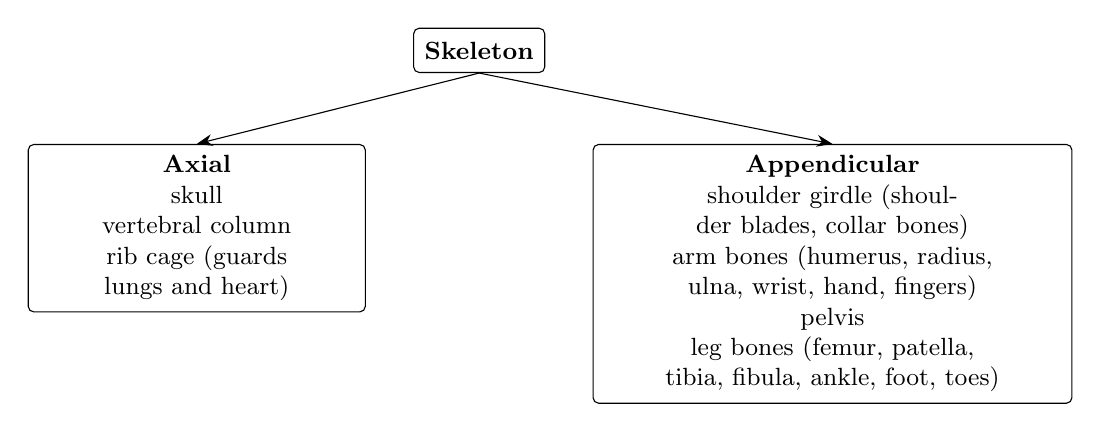
\begin{tikzpicture}
\node[head] (sk) {Skeleton};
\node[box, below left=9mm and 6mm of sk, text width=40mm] (ax) {\textbf{Axial}\\skull\\vertebral column\\rib cage (guards lungs and heart)};
\node[box, below right=9mm and 6mm of sk, text width=58mm] (ap) {\textbf{Appendicular}\\shoulder girdle (shoulder blades, collar bones)\\arm bones (humerus, radius, ulna, wrist, hand, fingers)\\pelvis\\leg bones (femur, patella, tibia, fibula, ankle, foot, toes)};
\draw[link] (sk.south) -- (ax.north);
\draw[link] (sk.south) -- (ap.north);
\end{tikzpicture}
\end{document}
